% Options for packages loaded elsewhere
\PassOptionsToPackage{unicode}{hyperref}
\PassOptionsToPackage{hyphens}{url}
%
\documentclass[
]{article}
\usepackage{amsmath,amssymb}
\usepackage{lmodern}
\usepackage{iftex}
\ifPDFTeX
  \usepackage[T1]{fontenc}
  \usepackage[utf8]{inputenc}
  \usepackage{textcomp} % provide euro and other symbols
\else % if luatex or xetex
  \usepackage{unicode-math}
  \defaultfontfeatures{Scale=MatchLowercase}
  \defaultfontfeatures[\rmfamily]{Ligatures=TeX,Scale=1}
\fi
% Use upquote if available, for straight quotes in verbatim environments
\IfFileExists{upquote.sty}{\usepackage{upquote}}{}
\IfFileExists{microtype.sty}{% use microtype if available
  \usepackage[]{microtype}
  \UseMicrotypeSet[protrusion]{basicmath} % disable protrusion for tt fonts
}{}
\makeatletter
\@ifundefined{KOMAClassName}{% if non-KOMA class
  \IfFileExists{parskip.sty}{%
    \usepackage{parskip}
  }{% else
    \setlength{\parindent}{0pt}
    \setlength{\parskip}{6pt plus 2pt minus 1pt}}
}{% if KOMA class
  \KOMAoptions{parskip=half}}
\makeatother
\usepackage{xcolor}
\usepackage[margin=1in]{geometry}
\usepackage{longtable,booktabs,array}
\usepackage{calc} % for calculating minipage widths
% Correct order of tables after \paragraph or \subparagraph
\usepackage{etoolbox}
\makeatletter
\patchcmd\longtable{\par}{\if@noskipsec\mbox{}\fi\par}{}{}
\makeatother
% Allow footnotes in longtable head/foot
\IfFileExists{footnotehyper.sty}{\usepackage{footnotehyper}}{\usepackage{footnote}}
\makesavenoteenv{longtable}
\usepackage{graphicx}
\makeatletter
\def\maxwidth{\ifdim\Gin@nat@width>\linewidth\linewidth\else\Gin@nat@width\fi}
\def\maxheight{\ifdim\Gin@nat@height>\textheight\textheight\else\Gin@nat@height\fi}
\makeatother
% Scale images if necessary, so that they will not overflow the page
% margins by default, and it is still possible to overwrite the defaults
% using explicit options in \includegraphics[width, height, ...]{}
\setkeys{Gin}{width=\maxwidth,height=\maxheight,keepaspectratio}
% Set default figure placement to htbp
\makeatletter
\def\fps@figure{htbp}
\makeatother
\setlength{\emergencystretch}{3em} % prevent overfull lines
\providecommand{\tightlist}{%
  \setlength{\itemsep}{0pt}\setlength{\parskip}{0pt}}
\setcounter{secnumdepth}{-\maxdimen} % remove section numbering
\usepackage{booktabs}
\usepackage{longtable}
\usepackage{array}
\usepackage{multirow}
\usepackage{wrapfig}
\usepackage{float}
\usepackage{colortbl}
\usepackage{pdflscape}
\usepackage{tabu}
\usepackage{threeparttable}
\usepackage{threeparttablex}
\usepackage[normalem]{ulem}
\usepackage{makecell}
\usepackage{xcolor}
\ifLuaTeX
  \usepackage{selnolig}  % disable illegal ligatures
\fi
\IfFileExists{bookmark.sty}{\usepackage{bookmark}}{\usepackage{hyperref}}
\IfFileExists{xurl.sty}{\usepackage{xurl}}{} % add URL line breaks if available
\urlstyle{same} % disable monospaced font for URLs
\hypersetup{
  pdftitle={Comparacion de Modelos para problema de Clasificación},
  pdfauthor={Área de Planificación Gestión y Estadística},
  hidelinks,
  pdfcreator={LaTeX via pandoc}}

\title{Comparacion de Modelos para problema de Clasificación}
\author{Área de Planificación Gestión y Estadística}
\date{2022-11-23}

\begin{document}
\maketitle

\hypertarget{introducciuxf3n}{%
\section{Introducción}\label{introducciuxf3n}}

En este estudio vamos a implementar tres modelos para clasificación de
clientes en ``buenos'' y ``malos'' pagadores a fin de su evaluación por
el BancoX.

\hypertarget{estructura-de-los-datos}{%
\section{Estructura de los datos}\label{estructura-de-los-datos}}

\begin{longtable}[]{@{}ll@{}}
\caption{Data summary}\tabularnewline
\toprule()
\endhead
Name & dataset \\
Number of rows & 500 \\
Number of columns & 10 \\
\_\_\_\_\_\_\_\_\_\_\_\_\_\_\_\_\_\_\_\_\_\_\_ & \\
Column type frequency: & \\
factor & 2 \\
numeric & 8 \\
\_\_\_\_\_\_\_\_\_\_\_\_\_\_\_\_\_\_\_\_\_\_\_\_ & \\
Group variables & None \\
\bottomrule()
\end{longtable}

\textbf{Variable type: factor}

\begin{longtable}[]{@{}
  >{\raggedright\arraybackslash}p{(\columnwidth - 10\tabcolsep) * \real{0.2000}}
  >{\raggedleft\arraybackslash}p{(\columnwidth - 10\tabcolsep) * \real{0.1429}}
  >{\raggedleft\arraybackslash}p{(\columnwidth - 10\tabcolsep) * \real{0.2000}}
  >{\raggedright\arraybackslash}p{(\columnwidth - 10\tabcolsep) * \real{0.1143}}
  >{\raggedleft\arraybackslash}p{(\columnwidth - 10\tabcolsep) * \real{0.1286}}
  >{\raggedright\arraybackslash}p{(\columnwidth - 10\tabcolsep) * \real{0.2143}}@{}}
\toprule()
\begin{minipage}[b]{\linewidth}\raggedright
skim\_variable
\end{minipage} & \begin{minipage}[b]{\linewidth}\raggedleft
n\_missing
\end{minipage} & \begin{minipage}[b]{\linewidth}\raggedleft
complete\_rate
\end{minipage} & \begin{minipage}[b]{\linewidth}\raggedright
ordered
\end{minipage} & \begin{minipage}[b]{\linewidth}\raggedleft
n\_unique
\end{minipage} & \begin{minipage}[b]{\linewidth}\raggedright
top\_counts
\end{minipage} \\
\midrule()
\endhead
Educacion & 0 & 1 & FALSE & 2 & 0: 346, 1: 154 \\
Default & 0 & 1 & FALSE & 2 & 0: 292, 1: 208 \\
\bottomrule()
\end{longtable}

\textbf{Variable type: numeric}

\begin{longtable}[]{@{}
  >{\raggedright\arraybackslash}p{(\columnwidth - 20\tabcolsep) * \real{0.1333}}
  >{\raggedleft\arraybackslash}p{(\columnwidth - 20\tabcolsep) * \real{0.0952}}
  >{\raggedleft\arraybackslash}p{(\columnwidth - 20\tabcolsep) * \real{0.1333}}
  >{\raggedleft\arraybackslash}p{(\columnwidth - 20\tabcolsep) * \real{0.0857}}
  >{\raggedleft\arraybackslash}p{(\columnwidth - 20\tabcolsep) * \real{0.0857}}
  >{\raggedleft\arraybackslash}p{(\columnwidth - 20\tabcolsep) * \real{0.0667}}
  >{\raggedleft\arraybackslash}p{(\columnwidth - 20\tabcolsep) * \real{0.0857}}
  >{\raggedleft\arraybackslash}p{(\columnwidth - 20\tabcolsep) * \real{0.0857}}
  >{\raggedleft\arraybackslash}p{(\columnwidth - 20\tabcolsep) * \real{0.0857}}
  >{\raggedleft\arraybackslash}p{(\columnwidth - 20\tabcolsep) * \real{0.0857}}
  >{\raggedright\arraybackslash}p{(\columnwidth - 20\tabcolsep) * \real{0.0571}}@{}}
\toprule()
\begin{minipage}[b]{\linewidth}\raggedright
skim\_variable
\end{minipage} & \begin{minipage}[b]{\linewidth}\raggedleft
n\_missing
\end{minipage} & \begin{minipage}[b]{\linewidth}\raggedleft
complete\_rate
\end{minipage} & \begin{minipage}[b]{\linewidth}\raggedleft
mean
\end{minipage} & \begin{minipage}[b]{\linewidth}\raggedleft
sd
\end{minipage} & \begin{minipage}[b]{\linewidth}\raggedleft
p0
\end{minipage} & \begin{minipage}[b]{\linewidth}\raggedleft
p25
\end{minipage} & \begin{minipage}[b]{\linewidth}\raggedleft
p50
\end{minipage} & \begin{minipage}[b]{\linewidth}\raggedleft
p75
\end{minipage} & \begin{minipage}[b]{\linewidth}\raggedleft
p100
\end{minipage} & \begin{minipage}[b]{\linewidth}\raggedright
hist
\end{minipage} \\
\midrule()
\endhead
N\_Cliente & 0 & 1 & 51933.90 & 29015.12 & 101.00 & 27152.00 & 52594.00
& 75916.50 & 99931.00 & ▆▇▆▇▇ \\
Edad & 0 & 1 & 33.54 & 12.57 & 18.00 & 24.00 & 30.00 & 40.00 & 77.00 &
▇▅▂▁▁ \\
Empleo & 0 & 1 & 6.58 & 8.54 & 0.00 & 0.00 & 3.00 & 10.00 & 51.00 &
▇▂▁▁▁ \\
Domicilio & 0 & 1 & 6.07 & 5.78 & 0.00 & 2.00 & 5.00 & 9.00 & 28.00 &
▇▃▁▁▁ \\
Ingreso & 0 & 1 & 58.69 & 58.60 & 14.00 & 27.00 & 40.00 & 64.00 & 512.00
& ▇▁▁▁▁ \\
Deuing & 0 & 1 & 10.42 & 7.08 & 0.20 & 4.90 & 9.15 & 13.75 & 36.60 &
▇▇▃▁▁ \\
Creddeu & 0 & 1 & 2.06 & 3.07 & 0.02 & 0.40 & 1.10 & 2.40 & 26.69 &
▇▁▁▁▁ \\
Otrdeu & 0 & 1 & 4.06 & 6.06 & 0.07 & 1.14 & 2.21 & 4.72 & 63.47 &
▇▁▁▁▁ \\
\bottomrule()
\end{longtable}

Vemos que no hay valores faltantes en los datos. Vemos que hay un
valores extremos que pueden afectar el desempeño de nuestros modelos,
sin perjuicio de lo cual mantendremos las observaciones para corroborar
si alguno de ellos resiste estas particularidades en los datos sin
eliminar observaciones. Incluimos N\_Cliente pese a ser variable
indentificatoria por simple interés de revisión de la consistencia de
las bases de datos.

\hypertarget{distribuciones-y-correlaciones}{%
\section{Distribuciones y
correlaciones}\label{distribuciones-y-correlaciones}}

\includegraphics{Parcial2_AE_files/figure-latex/unnamed-chunk-2-1.pdf}

Como vemos la variable Deuing contiene información de utilidad para la
clasificación que estamos intentando realizar, como así tambien la
variable Empleo y Domicilio (estas variables pueden ser colineales).
Cabe notar que consideradas individualmente las variables tienen muchos
outlier.

\hypertarget{gruxe1fico-con-variables-de-interuxe9s}{%
\subsection{Gráfico con variables de
interés}\label{gruxe1fico-con-variables-de-interuxe9s}}

\begin{center}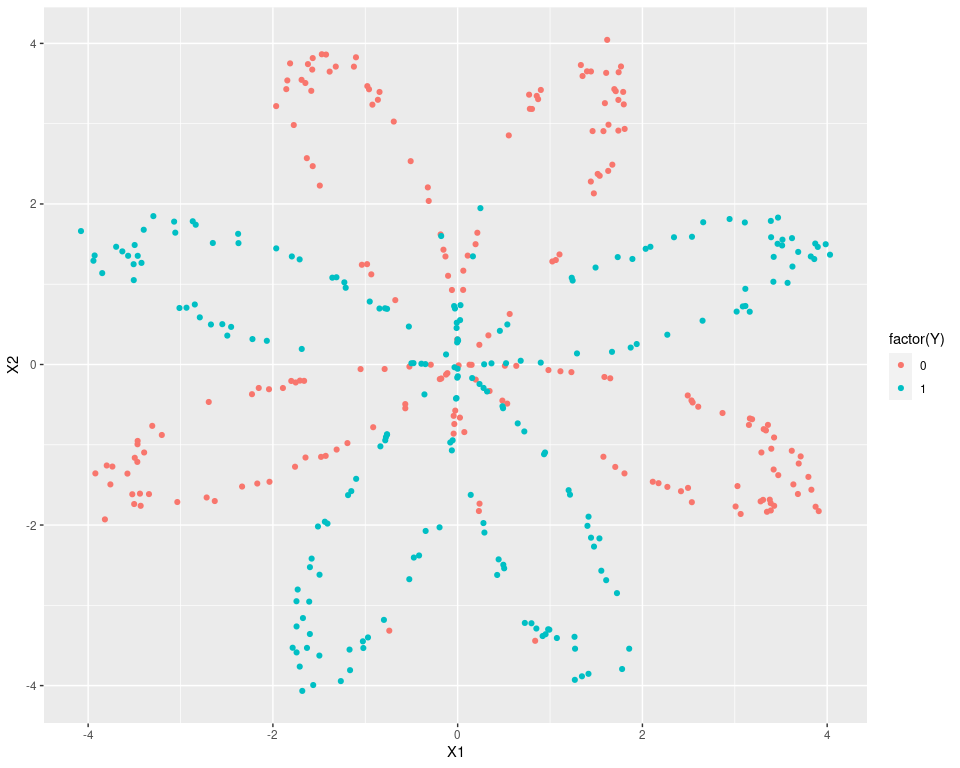
\includegraphics{Parcial2_AE_files/figure-latex/unnamed-chunk-3-1} \end{center}

A continuación plantearemos tres modelos para este problema.

\hypertarget{regresion-loguxedstica}{%
\section{Regresion logística}\label{regresion-loguxedstica}}

\hypertarget{modelo-simple}{%
\subsubsection{Modelo Simple}\label{modelo-simple}}

\begin{verbatim}
## parsnip model object
## 
## 
## Call:  stats::glm(formula = Default ~ Deuing, family = stats::binomial, 
##     data = data)
## 
## Coefficients:
## (Intercept)       Deuing  
##     -1.6940       0.1285  
## 
## Degrees of Freedom: 499 Total (i.e. Null);  498 Residual
## Null Deviance:       679 
## Residual Deviance: 598   AIC: 602
\end{verbatim}

\hypertarget{modelo-completo}{%
\subsubsection{Modelo Completo}\label{modelo-completo}}

Plateamos el modelo completo con todas las variables. El procesamiento
crea automáticamente la variable dummy a partir de ``Educación''.
Intentamos un modelo multiple utilizando predictoras a \emph{Empleo +
Deuing + Creddeu} pero descartamos esta fórmula para emplear todas las
variables -como se muestra seguidamente- porque arrojan mejor resultado
de Devianza y AIC.

\begin{verbatim}
## parsnip model object
## 
## 
## Call:  stats::glm(formula = Default ~ ., family = stats::binomial, data = data)
## 
## Coefficients:
## (Intercept)    N_Cliente         Edad   Educacion1       Empleo    Domicilio  
##  -7.100e-01   -6.995e-07   -1.591e-02    3.930e-01   -2.109e-01   -1.267e-01  
##     Ingreso       Deuing      Creddeu       Otrdeu  
##   2.593e-03    1.197e-01    5.843e-01    7.808e-04  
## 
## Degrees of Freedom: 499 Total (i.e. Null);  490 Residual
## Null Deviance:       679 
## Residual Deviance: 434.4     AIC: 454.4
\end{verbatim}

\hypertarget{comparando-modelos-loguxedsticos}{%
\subsubsection{Comparando modelos
logísticos}\label{comparando-modelos-loguxedsticos}}

\begin{verbatim}
## # A tibble: 2 x 3
##   Model             AIC   BIC
##   <chr>           <dbl> <dbl>
## 1 modelo completo  454.  497.
## 2 modelo simple    602.  610.
\end{verbatim}

Vemos que el modelo completo tiene \emph{BIC} y un \emph{AIC} menor que
el modelo simple. Ahora veremos los p\_valores por predictor:

\begin{verbatim}
## 
## Call:
## stats::glm(formula = Default ~ ., family = stats::binomial, data = data)
## 
## Deviance Residuals: 
##     Min       1Q   Median       3Q      Max  
## -2.2438  -0.7492  -0.1426   0.7231   2.3595  
## 
## Coefficients:
##               Estimate Std. Error z value Pr(>|z|)    
## (Intercept) -7.100e-01  7.653e-01  -0.928   0.3535    
## N_Cliente   -6.995e-07  4.141e-06  -0.169   0.8659    
## Edad        -1.591e-02  3.380e-02  -0.471   0.6378    
## Educacion1   3.930e-01  2.741e-01   1.434   0.1516    
## Empleo      -2.109e-01  4.027e-02  -5.236 1.64e-07 ***
## Domicilio   -1.267e-01  7.702e-02  -1.645   0.0999 .  
## Ingreso      2.593e-03  5.671e-03   0.457   0.6475    
## Deuing       1.197e-01  3.042e-02   3.936 8.30e-05 ***
## Creddeu      5.843e-01  1.177e-01   4.963 6.93e-07 ***
## Otrdeu       7.808e-04  5.147e-02   0.015   0.9879    
## ---
## Signif. codes:  0 '***' 0.001 '**' 0.01 '*' 0.05 '.' 0.1 ' ' 1
## 
## (Dispersion parameter for binomial family taken to be 1)
## 
##     Null deviance: 678.97  on 499  degrees of freedom
## Residual deviance: 434.36  on 490  degrees of freedom
## AIC: 454.36
## 
## Number of Fisher Scoring iterations: 6
\end{verbatim}

\hypertarget{tabla-de-resultados-de-clasificaciuxf3n-loguxedstica}{%
\subsubsection{Tabla de Resultados de clasificación
logística}\label{tabla-de-resultados-de-clasificaciuxf3n-loguxedstica}}

\includegraphics{Parcial2_AE_files/figure-latex/unnamed-chunk-9-1.pdf}

\hypertarget{exactitud-del-modelo-loguxedstico}{%
\subsubsection{Exactitud del modelo
logístico}\label{exactitud-del-modelo-loguxedstico}}

\begin{verbatim}
## # A tibble: 1 x 3
##   .metric  .estimator .estimate
##   <chr>    <chr>          <dbl>
## 1 accuracy binary         0.782
\end{verbatim}

\hypertarget{red-bayesiana}{%
\section{Red Bayesiana}\label{red-bayesiana}}

\hypertarget{ajuste-del-modelo}{%
\subsubsection{Ajuste del modelo}\label{ajuste-del-modelo}}

\begin{verbatim}
## parsnip model object
## 
## $apriori
## grouping
##     0     1 
## 0.584 0.416 
## 
## $tables
## $tables$N_Cliente
##       [,1]     [,2]
## 0 52186.00 28788.05
## 1 51579.99 29396.93
## 
## $tables$Edad
##       [,1]      [,2]
## 0 36.76027 13.495986
## 1 29.01923  9.474074
## 
## $tables$Educacion
##         var
## grouping        0        1
##        0 0.739726 0.260274
##        1 0.625000 0.375000
## 
## $tables$Empleo
##       [,1]     [,2]
## 0 8.609589 9.372309
## 1 3.725962 6.191540
## 
## $tables$Domicilio
##       [,1]     [,2]
## 0 7.527397 6.314980
## 1 4.033654 4.170731
## 
## $tables$Ingreso
##       [,1]     [,2]
## 0 61.60274 58.19377
## 1 54.59135 59.06994
## 
## $tables$Deuing
##        [,1]     [,2]
## 0  8.080137 5.437930
## 1 13.700481 7.793398
## 
## $tables$Creddeu
##       [,1]     [,2]
## 0 1.426370 1.744121
## 1 2.953125 4.135714
## 
## $tables$Otrdeu
##       [,1]     [,2]
## 0 3.434589 4.249271
## 1 4.940913 7.857593
## 
## 
## $levels
## [1] "0" "1"
## 
## $call
## NaiveBayes.default(x = ~maybe_data_frame(x), grouping = ~y, usekernel = ~FALSE)
## 
## $x
##     N_Cliente Edad Educacion Empleo Domicilio Ingreso Deuing Creddeu Otrdeu
## 1       97175   77         1      2        24      28   10.6    1.37   1.60
## 2       89611   37         1      0         9      83   14.9    5.90   6.47
## 3       39391   35         1      9         6     123    6.1    1.70   5.80
## 4       59445   24         1      0         0      64   13.0    3.98   4.34
## 5       98293   31         1      1         4      43    7.9    2.49   0.90
## 6       64828   59         1     19        21     174   27.9   16.41  32.14
## 7        5146   18         0      0         0      27    4.1    0.17   0.94
## 8       76141   29         0      8         5      35   21.1    1.65   5.73
## 9       50081   38         1      6         7      25   31.3    2.21   5.61
## 10      95329   27         0      3         5      26    2.0    0.04   0.48
## 11      14435   49         0     15        11      35    3.0    0.74   0.32
## 12      20424   24         0      1         2      23   14.8    0.80   2.61
## 13      14754   27         1      3         5      36   16.2    1.39   4.44
## 14      41624   26         0      2         4      26   14.5    0.56   3.21
## 15       7648   32         1      0         6      37    3.1    0.59   0.55
## 16      68341   53         1     16        13      51    4.1    0.95   1.14
## 17      99760   19         0      0         0      17   14.1    1.04   1.36
## 18      50562   18         0      0         0      19    6.4    0.40   0.82
## 19      68173   19         0      1         0      21    7.9    1.10   0.55
## 20      73205   51         0     25        16      96   21.5    7.31  13.33
## 21      58135   30         1      3         2      40   16.9    2.22   4.54
## 22      79853   63         0     22        21      61   13.5    1.83   6.41
## 23      19891   30         1      1         4      73   29.8    7.05  14.71
## 24      58639   27         1      3         3      43    4.5    0.58   1.36
## 25      96165   42         0     15         9      46   13.1    1.06   4.97
## 26      70000   24         1      0         3      44   13.5    2.38   3.56
## 27      67462   20         0      0         0      23   23.6    3.54   1.89
## 28      43432   28         0      4         5      20    6.2    0.57   0.67
## 29      86490   25         0      3         2      23    5.0    0.28   0.87
## 30      11308   24         1      0         3      49    5.0    0.87   1.58
## 31      13785   36         0      9         7      76    5.7    0.29   4.04
## 32      35484   44         0     11        12      50   22.0    2.11   8.89
## 33      53570   23         0      0         1      45   15.8    1.12   5.99
## 34      89434   32         0      1         4      26    3.3    0.24   0.62
## 35      10830   32         0      9         7      53   14.9    5.81   2.08
## 36      56215   35         1      7         6      76    7.0    0.56   4.76
## 37      40101   30         0      3         6      34   14.3    2.26   2.61
## 38      24775   30         0      4         3      36    9.6    0.83   2.63
## 39      80786   31         0      6         5      26    6.5    0.33   1.36
## 40      70691   23         0      0         2      16   17.2    0.91   1.84
## 41       1909   46         0     11         8      61   10.4    3.44   2.90
## 42      20474   59         0     33        17     308    6.7    7.39  13.25
## 43      70135   39         1      1        10     185    7.0   10.45   2.50
## 44      20766   29         1      3         3      55   27.1    8.35   6.56
## 45      64636   26         1      2         4      19    3.8    0.11   0.62
## 46       7844   34         0      6         7      27    6.4    0.27   1.46
## 47      54870   30         0     12         5      35    5.7    1.34   0.66
## 48       5878   23         1      0         2      29    9.4    0.84   1.89
## 49      12502   22         1      0         1      76    7.7    3.62   2.24
## 50      16260   27         1      0         4      46    1.9    0.23   0.64
## 51        101   30         0      0         5      70    6.9    0.37   4.46
## 52      26980   23         0      0         1      22    9.0    0.71   1.27
## 53      28480   42         1     12        13      34    6.1    0.56   1.52
## 54      97068   29         1      2         3      55   15.6    1.48   7.10
## 55      11228   47         0     16         8      66    1.7    0.10   1.02
## 56      34771   34         1      8         7      30    5.7    1.08   0.63
## 57      22992   31         0     11         7      51   12.4    4.14   2.19
## 58      68333   35         1     10         4      53   19.0    3.64   6.43
## 59      25246   19         0      2         0      21   12.0    0.15   2.37
## 60      88239   30         0      7         7      40   11.4    1.78   2.78
## 61      96992   25         1      0         2      35    0.6    0.07   0.14
## 62      64980   38         1     11         8      40    8.8    1.65   1.87
## 63      19289   18         0      0         0      34    2.8    0.29   0.66
## 64      60645   53         0     10        14      62   13.4    2.38   5.93
## 65      19737   31         0     10         5      60   27.3    6.27  10.11
## 66      72222   38         1      7         7     274    2.3    4.32   1.99
## 67      64856   19         0      0         0      21    2.5    0.03   0.49
## 68      95167   20         0      2         0      18    2.3    0.06   0.36
## 69      97757   21         0      2         1      22    9.2    1.05   0.98
## 70      49564   19         0      0         0      17    5.5    0.51   0.43
## 71      72439   23         1      0         1      42   12.2    2.24   2.88
## 72      28087   65         0     25        20      48    7.7    2.81   0.88
## 73      93596   45         1     18        12      88    9.6    4.04   4.41
## 74      22255   21         0      0         1      22    1.5    0.10   0.23
## 75      11363   54         0      8        10      67   10.5    1.25   5.79
## 76      14488   22         1      0         2      24    8.0    0.64   1.28
## 77      93279   20         0      0         0      23   14.2    1.86   1.40
## 78      31083   41         0     12         9      58   13.1    3.78   3.81
## 79      51227   36         0     14         3      71    6.9    1.43   3.47
## 80      98608   33         0     11         8      79   10.8    3.08   5.45
## 81       9416   23         0      2         2      34    3.3    0.22   0.90
## 82      17970   46         0      8         6     119    5.6    1.11   5.55
## 83      13419   21         0      0         0      15    6.1    0.07   0.84
## 84      96496   28         1      2         4      62   34.8    3.86  17.71
## 85      93765   39         0      9         8      69    6.0    0.55   3.59
## 86      78339   54         1      4         9      69   12.0    1.18   7.10
## 87       1329   75         0     22        23      56    7.8    1.79   2.58
## 88      86302   31         1      1         7      69    0.4    0.19   0.09
## 89      74530   55         0     32         8     229    4.9    3.03   8.19
## 90      67259   20         0      0         0      18   17.4    0.42   2.71
## 91      17141   39         1      3         9      42   15.2    3.08   3.31
## 92      51379   37         0      2         8      55    8.0    1.64   2.76
## 93      12618   20         0      0         0      41    4.3    0.47   1.29
## 94      12278   57         1     10        10     149   10.0    3.64  11.26
## 95      11413   50         0     20        15     117    7.6    3.15   5.74
## 96      24334   33         0      2         7      28    1.6    0.14   0.31
## 97      72925   36         0     16        10      44    7.4    1.96   1.30
## 98      69122   21         0      1         0      29    5.7    0.64   1.01
## 99      39430   37         0     12        11     121   13.6    4.69  11.77
## 100     53336   27         1      0         4      24    6.1    0.17   1.30
## 101     32861   28         1      5         5     112    9.9    0.93  10.16
## 102     37115   27         0      4         5      40   13.2    3.73   1.55
## 103     55036   32         0      4         3      37    4.1    0.48   1.04
## 104     49591   28         0      6         5      33   20.5    1.10   5.67
## 105     65383   24         1      0         2      35   12.1    2.47   1.77
## 106     67716   20         0      0         0      44    3.9    1.07   0.65
## 107     97591   39         1     16         4      47   16.5    4.16   3.60
## 108     81476   38         1     11         8     145   18.5    1.45  25.38
## 109     91524   65         0     38        11     352    2.5    0.39   8.41
## 110     97604   56         0     34        19     215   13.9   14.37  15.51
## 111     49015   18         0      0         0      57    3.1    1.24   0.53
## 112     27067   20         0      0         1      18    9.5    0.16   1.55
## 113     83322   62         0      4        13      27   13.2    1.73   1.84
## 114     10086   39         0     13         8     112   21.2    4.63  19.11
## 115     23978   29         1      3         2     102    9.8    4.83   5.17
## 116     64810   30         1      4         6      46    3.9    1.26   0.54
## 117     72868   52         0     21        14     121    2.4    0.39   2.51
## 118     59632   48         1     19        11     326   10.6   21.18  13.37
## 119     51088   20         0      2         0      42    3.1    0.89   0.41
## 120     43145   34         1      7         3      33    7.5    1.88   0.60
## 121     16884   68         0     51        26     274    7.0    8.59  10.59
## 122     27155   47         0     16        15      51   14.2    3.40   3.85
## 123     93646   37         0     12         8      29    9.3    0.88   1.82
## 124     11258   36         0      9        10      35    0.8    0.09   0.19
## 125     17298   30         1      1         6     107    8.9    1.44   8.09
## 126     41655   24         0      0         2      21   13.7    1.38   1.50
## 127     96020   24         1      0         2      49   13.6    3.04   3.63
## 128     65856   31         0      0         6      34    4.2    0.71   0.71
## 129     21601   41         1     15        13      89    9.2    2.55   5.63
## 130     15914   19         0      0         0      25   24.7    1.23   4.95
## 131     79675   20         0      0         1      23    1.0    0.02   0.21
## 132     73735   30         0      8         5      65    9.2    2.45   3.53
## 133      8853   42         0      5        12      72   19.3    0.25  13.65
## 134     13968   27         0      5         5      34    1.0    0.06   0.28
## 135     21565   24         1      0         2      38    1.6    0.03   0.57
## 136     67101   38         0     16         6      71    6.6    1.54   3.15
## 137      3110   24         0      7         2      29   13.6    0.64   3.30
## 138     83360   48         0      7        11      80    3.7    0.79   2.17
## 139     88021   49         1      0        11      77    2.0    0.21   1.33
## 140     57638   18         0      0         0      29   25.9    2.39   5.12
## 141     89037   64         0     11        28      27    2.4    0.08   0.57
## 142     23405   19         0      3         0      22   10.9    0.47   1.93
## 143     14713   49         0      2        17      36   23.6    2.66   5.84
## 144     42530   29         1      1         4      26    6.6    0.51   1.21
## 145     46708   28         0      3         5      64    9.4    1.03   4.98
## 146     47166   27         0      4         3      32    6.7    0.56   1.59
## 147     32952   24         1      0         2      40    8.6    1.20   2.24
## 148     73333   23         0      2         2      38   12.2    2.23   2.41
## 149     99435   43         1      3         8      30    3.1    0.34   0.59
## 150     80926   29         1      1         5      51   12.5    2.43   3.95
## 151     88937   61         0     35         9     327    4.6    7.63   7.42
## 152     41754   22         1      0         1      20    6.5    0.60   0.70
## 153     57674   24         0      2         3      34    2.4    0.27   0.54
## 154     46567   30         0      8         3      65    8.8    1.92   3.80
## 155     65026   37         0      3         4      57   10.8    0.72   5.44
## 156     95015   27         0      4         1      36   14.7    1.46   3.83
## 157     19954   22         1      0         1      29    3.7    0.08   0.99
## 158     96517   28         1      1         3      77    0.2    0.06   0.10
## 159     66589   31         0     11         4      41    2.0    0.34   0.48
## 160      8965   44         0     14        12      68   14.9    1.78   8.35
## 161     30209   69         0     24        22      84   20.2    5.63  11.33
## 162     79504   26         0      5         2      42   10.6    2.13   2.32
## 163     15574   51         0      9        15      96   16.8    0.58  15.55
## 164     60298   20         0      0         0      77    9.6    3.85   3.54
## 165     66331   24         0      2         0      43    7.3    1.24   1.90
## 166     33249   53         0     17         9      59    0.5    0.03   0.26
## 167     95765   29         0      0         4      28    4.7    0.14   1.18
## 168       547   52         0     28        16     368   21.3   24.06  54.32
## 169     90253   28         0      4         4      20   21.1    0.57   3.65
## 170     97919   35         0     17         5     160   13.5    9.07  12.53
## 171     66528   20         0      0         0      27   10.3    0.39   2.39
## 172     42444   27         1      0         3      36    4.1    0.73   0.75
## 173     27555   34         1      2         4      46   22.5    1.21   9.14
## 174     18807   46         1     13        14      84    9.9    1.71   6.60
## 175     89002   36         1      4         8     101    6.7    2.09   4.68
## 176     92675   51         1      4         6      43    3.3    0.20   1.22
## 177     47914   39         0     20        10      52   19.7    2.33   7.92
## 178     99931   33         1      4         6      24   27.7    3.20   3.44
## 179     78146   65         0     38        25     231    9.3    2.02  19.46
## 180     47058   35         0     10         8     263    4.9    9.27   3.62
## 181     63295   41         0     22         7     226   17.4    7.12  32.21
## 182     55049   23         0      0         1      33    1.7    0.24   0.32
## 183     71544   23         0      5         1      23   24.3    3.50   2.08
## 184     55437   34         1      0         5     120    6.4    5.55   2.13
## 185     99810   18         0      0         0      30   19.8    2.30   3.64
## 186     38160   29         1      3         2      26    7.8    0.46   1.57
## 187     50923   38         1     13        12     204   19.5   15.43  24.35
## 188     73111   32         1      8         5      44   13.7    1.35   4.68
## 189      8650   34         0     12         7      58   19.9    2.49   9.05
## 190     84368   37         0     14         4      67   13.4    2.12   6.86
## 191     58187   37         0      4         6      53   15.5    1.27   6.95
## 192     35254   37         0      4         6      30    4.6    0.71   0.67
## 193     34519   45         1     16        13      53    5.7    0.93   2.09
## 194     29255   48         0      4        12      57   12.1    2.46   4.43
## 195      5203   36         0     12         5      55    5.8    1.20   1.99
## 196     90447   26         0      1         3      42    1.5    0.08   0.55
## 197     93989   60         0     31        22     170    8.0    8.77   4.83
## 198     52731   37         0      2         9      31    9.6    1.54   1.44
## 199     70627   27         1      1         2      21   14.4    0.52   2.51
## 200     47169   26         0      6         2      46    9.8    0.34   4.17
## 201     71115   32         0      7         5      34   10.7    0.52   3.12
## 202     72268   23         0      0         1      16    7.8    0.35   0.90
## 203     31560   58         0     18        13      54    4.2    0.82   1.45
## 204     69688   34         0      0         7      26    1.9    0.18   0.32
## 205     69814   30         0      0         4      17    4.9    0.41   0.42
## 206     26794   25         0      2         3      52    7.7    1.07   2.93
## 207     28684   24         0      3         2      24   10.7    1.98   0.59
## 208     22086   34         1      1         7      40   17.6    1.68   5.36
## 209     67315   64         0      7        26      24    6.5    0.29   1.27
## 210     39766   29         1      2         5      34   19.0    1.03   5.43
## 211     20804   21         0      1         1      29    0.9    0.02   0.24
## 212     20731   50         1      9        11      24   15.7    0.58   3.18
## 213     39028   25         1      0         2      29   15.7    1.83   2.73
## 214     85237   27         0      6         5      20   13.2    1.44   1.20
## 215     12795   25         0      4         3      41   18.4    2.01   5.54
## 216     13368   27         1      3         5      41    4.8    0.55   1.41
## 217     49943   26         0      4         4      31    5.5    0.25   1.45
## 218     96805   49         0      6        12      49    1.7    0.50   0.33
## 219     40533   41         0      0         8      39   29.1    2.16   9.19
## 220     55658   30         0      4         2      55    5.5    1.45   1.57
## 221     94403   37         0     16         8      43    5.6    0.64   1.77
## 222      9263   34         0      9         3      62    8.0    0.40   4.56
## 223     22644   50         1     23        11     104    4.8    0.93   4.06
## 224     81468   28         0      4         2      58   12.6    2.48   4.83
## 225     96758   19         0      0         0      20    3.1    0.26   0.36
## 226     32407   25         1      0         1      31    3.9    0.37   0.84
## 227     70940   18         0      0         0      15   12.2    0.37   1.46
## 228     45285   24         1      0         2      32    5.6    0.25   1.54
## 229      4217   30         0      5         6      26   14.8    0.97   2.87
## 230     78870   36         0      1         4      55   19.6    6.36   4.42
## 231     22101   32         1      0         5      38    3.7    0.18   1.22
## 232     96039   41         1      2         7      94    7.0    1.16   5.42
## 233     27143   47         0     28        11     189    3.2    4.18   1.87
## 234     80756   57         0     26        22      78    5.8    1.24   3.28
## 235     89436   26         0      4         3      34   19.0    0.67   5.79
## 236     12714   34         1      6         5      65   14.4    4.98   4.38
## 237     14519   33         0      0         7      64   10.6    2.69   4.10
## 238     31004   53         1      9        11      97   22.3    9.21  12.42
## 239      5641   61         0     20        17      91    4.3    1.26   2.65
## 240     80560   18         0      0         0      14    4.3    0.15   0.45
## 241      4017   21         0      0         1      18   12.1    0.59   1.59
## 242     65460   28         0      7         2      52   22.1    6.78   4.71
## 243     91095   34         0      4         8      49    3.1    0.04   1.48
## 244     36031   20         0      2         0      16    4.7    0.25   0.50
## 245     29387   34         0     11         6      54   10.6    3.12   2.60
## 246      3992   22         0      0         1      14    2.5    0.26   0.09
## 247     57232   34         0      8         7      30   24.3    0.21   7.08
## 248     85402   18         0      0         0      18   13.1    0.92   1.44
## 249     12337   41         0     21         9      64    0.3    0.12   0.07
## 250     64707   46         0      4         7      67    3.4    0.76   1.52
## 251     63714   21         0      0         1      20    2.2    0.10   0.34
## 252     31966   51         0     19        16      47   22.7    3.28   7.39
## 253     70991   27         1      0         3      25   22.9    1.09   4.64
## 254     42607   35         0     15         3      30   21.3    1.28   5.11
## 255     73833   22         1      0         2      26    6.0    0.02   1.54
## 256     71515   65         0     38        13     143   11.1    1.17  14.70
## 257     10482   43         0      5        11      27   21.2    2.83   2.90
## 258     62151   23         1      0         2      23   18.0    0.51   3.63
## 259     42352   66         0     43        22     152    9.0    5.06   8.62
## 260     74770   25         0      3         2      48    8.2    2.87   1.07
## 261     48829   35         1      0        11      84    3.4    1.18   1.67
## 262     67236   19         0      0         0      20   12.8    1.14   1.42
## 263     61485   25         1      1         1      20    6.9    0.43   0.95
## 264     30398   23         1      0         1      62    3.0    0.56   1.30
## 265     92578   23         0      2         1      40   21.2    2.65   5.83
## 266     18936   49         0     12        11      85    4.5    2.29   1.53
## 267     95835   45         1      6        10      59   10.6    3.80   2.45
## 268     91698   45         0     10        13      45    2.9    0.19   1.12
## 269     79388   32         1      6         7      31    5.2    0.38   1.23
## 270     36804   28         1      0         4      60    0.5    0.08   0.22
## 271     11314   44         0     22         9     131    7.0    0.83   8.34
## 272     63037   49         0     20         9     140    9.9    4.42   9.44
## 273     43472   19         0      0         0      19    4.4    0.06   0.77
## 274     45710   34         0      0         6      24    9.4    0.08   2.18
## 275     36648   51         0      2        15      34    7.2    1.77   0.68
## 276     69984   28         0      4         4      25   34.8    1.04   7.66
## 277     41904   51         1     20        18     512    6.5    6.82  26.46
## 278     24918   24         1      0         1      63   26.9    7.19   9.76
## 279     78220   41         1      9        14      87    4.4    0.78   3.05
## 280     37120   23         1      0         1      35   15.0    0.40   4.85
## 281     97700   33         1      3         7      19   17.2    0.37   2.90
## 282     32499   42         0     18         5     176    5.6    3.91   5.94
## 283     96131   20         0      0         0      16    3.5    0.23   0.33
## 284     46245   27         0      3         4      26    2.6    0.09   0.58
## 285     55485   34         0      9         3      29   11.6    1.06   2.30
## 286     86766   20         0      0         0      34   12.9    0.90   3.49
## 287     40033   66         0      9        23      54   15.8    1.34   7.19
## 288     33409   19         0      0         0      20   12.7    1.22   1.32
## 289     34885   33         1      2         7      79   23.7   10.47   8.26
## 290     55912   22         0      1         1      17   25.4    2.38   1.94
## 291      6275   40         0      5         7      43   23.9    3.69   6.59
## 292     62873   55         1     25        12      73   19.1    5.80   8.14
## 293     89597   25         1      1         1      15    8.9    0.56   0.78
## 294     99284   23         0      0         1      30    6.9    0.55   1.52
## 295      4834   37         1     13         5     225    1.1    1.42   1.06
## 296     90701   18         0      0         0      21    6.6    0.08   1.31
## 297       292   23         0      4         1      22    3.8    0.08   0.76
## 298     29607   27         0      2         2      55   11.7    0.54   5.89
## 299     37909   42         1      6         8      20   15.3    1.43   1.63
## 300     88393   31         0      9         6      23    7.8    0.45   1.35
## 301     25065   33         0      9         5      34   12.7    3.16   1.16
## 302     21016   58         1     26        21     132    2.4    0.98   2.19
## 303     57875   58         0     24        24     138    3.9    2.86   2.52
## 304     91654   48         0     12        12      51    4.3    0.22   1.97
## 305     80263   26         0      2         4      55   11.0    4.69   1.36
## 306      9231   28         1      2         5      18   11.9    0.32   1.82
## 307     67262   22         0      4         1      21    9.0    0.87   1.02
## 308     86248   18         0      0         0      18    8.0    0.40   1.04
## 309     87126   57         0      4        12      61    2.3    0.11   1.29
## 310      5097   19         0      1         0      24   12.3    1.11   1.84
## 311     44891   31         1      4         5      36   22.4    0.15   7.91
## 312     50200   18         0      1         0      18    8.0    0.74   0.70
## 313     95980   23         0      0         1      18    4.0    0.05   0.67
## 314     45451   19         0      0         0      14    8.2    0.38   0.77
## 315      7679   29         0      0         4      70   16.5    8.21   3.34
## 316     64910   29         0      8         5      39   11.6    3.26   1.27
## 317     71392   25         0      2         3      24    3.0    0.15   0.57
## 318     49338   18         0      0         0      24    0.9    0.13   0.09
## 319     15306   40         0      4         6      87    1.2    0.86   0.18
## 320     97311   31         0     11         8      36    4.7    0.13   1.57
## 321     37305   52         1      2        12      84    3.1    0.20   2.40
## 322     96590   37         0     18         3      39   26.9    5.46   5.04
## 323     64889   40         0     18        13      84    6.2    0.94   4.27
## 324     18301   18         0      0         0      17   11.9    0.17   1.86
## 325     79696   45         0     24        14      69    3.2    1.33   0.87
## 326     55845   34         0     11         6      52   12.9    4.17   2.54
## 327     44591   19         0      0         0      21   12.6    1.23   1.42
## 328     41159   25         0      3         1      27   16.9    1.09   3.48
## 329     61614   53         0     30        12     220   12.9    2.81  25.57
## 330     96725   30         0      4         4      39   11.6    1.39   3.13
## 331     37549   49         1     23        11     178   19.4    5.59  28.94
## 332     97649   21         0      2         1      23    3.5    0.25   0.55
## 333     58830   40         0      0        12      21   36.6    4.35   3.34
## 334     12446   18         0      0         0      23   11.5    0.66   1.98
## 335     63892   18         0      0         0      15    8.0    0.22   0.98
## 336     20124   34         0     10         6      50    5.3    0.58   2.07
## 337     86824   33         1      5         8      27   20.6    1.09   4.47
## 338     92828   45         0     23        10      55   13.3    1.46   5.86
## 339     30248   40         1     15        13     111    9.6    1.88   8.78
## 340     54058   49         0      4        11      36    9.9    1.36   2.21
## 341     68265   27         0      0         4      31    3.7    0.28   0.86
## 342     27415   52         0     26        12      77   28.6    5.26  16.76
## 343     32685   23         0      1         2      30   18.2    1.37   4.09
## 344     98596   39         0     16        10      46   11.3    1.45   3.75
## 345     36195   20         0      0         1      28    9.8    0.66   2.09
## 346     87253   26         0      0         3      23   10.9    1.71   0.80
## 347     14781   62         1     23        22     124   23.0   19.05   9.47
## 348     35148   39         0      1         9      27    1.4    0.10   0.28
## 349      1874   26         0      5         2      47   21.7    6.14   4.06
## 350     38212   35         0     15         8      66    3.3    1.05   1.12
## 351     48520   46         1     11         9     136    4.9    3.27   3.39
## 352     37280   47         1     17        17      61    7.5    3.12   1.45
## 353     94442   56         0      3        16      38   18.7    3.72   3.39
## 354     26206   21         0      0         1      33    9.1    1.05   1.95
## 355     93422   29         0      0         5      33    5.8    0.58   1.34
## 356     93164   28         0      3         5      53    5.7    1.57   1.45
## 357     67271   28         0      3         3      61   16.1    3.16   6.66
## 358     61108   30         0      4         6      30   10.8    1.03   2.21
## 359     20134   20         0      1         0      22   10.1    0.14   2.08
## 360     10049   24         1      0         2      29    9.6    1.04   1.75
## 361     75133   29         1      5         4      73   25.1    2.18  16.14
## 362     10645   19         0      0         0      15    9.5    0.40   1.03
## 363     63862   63         0     29        19     208   16.6   21.89  12.64
## 364     91145   39         0     17         9      90    6.8    3.45   2.67
## 365     61110   22         1      0         1      30    3.4    0.15   0.87
## 366     10909   30         0      2         4      34   11.6    1.39   2.55
## 367     29547   24         0      4         2      24   18.0    1.64   2.68
## 368     97862   25         1      1         2      66    4.2    0.55   2.22
## 369     80518   22         0      2         1      39    4.7    0.50   1.33
## 370     49797   35         1      0         9      36   13.3    0.99   3.80
## 371     25377   51         0     14        16     161    1.4    0.57   1.69
## 372     82252   65         0      0        25      57    6.2    1.68   1.86
## 373     38077   38         1     14         7     192   28.9    5.27  50.22
## 374     11008   28         0      8         4      24   24.6    4.07   1.83
## 375     92555   30         1      2         5      27   10.6    0.74   2.13
## 376     43526   22         1      0         2      46    8.6    1.76   2.19
## 377     84423   19         0      0         0      28    7.5    1.51   0.59
## 378     47231   48         1     24        18      66    4.4    0.32   2.58
## 379     18015   18         0      0         0      16    8.3    0.17   1.15
## 380     86518   29         0      1         5      39   10.3    2.98   1.03
## 381     30441   37         0      0         9      37   16.2    0.93   5.06
## 382     20752   23         1      0         1      73    0.7    0.25   0.26
## 383     26249   27         0      4         5      41    6.1    1.65   0.85
## 384     42908   38         1     10        11      63   12.2    2.76   4.93
## 385      3688   39         0     10         7      45   25.0    1.77   9.48
## 386     61193   28         1      4         3      48   24.3    3.34   8.33
## 387     61148   54         0      2        19      35    6.4    0.93   1.31
## 388     55904   39         1     12        10      98    1.6    0.16   1.41
## 389     28778   19         0      0         0      26   17.2    2.65   1.82
## 390     96650   71         0      2        13      23   10.1    1.44   0.89
## 391     59227   24         0      4         2      21    3.8    0.36   0.44
## 392     83101   28         0      3         4      20    9.0    0.37   1.43
## 393     65132   21         0      4         1      15    7.3    0.05   1.04
## 394     50600   36         0      8         2      42    3.1    0.75   0.55
## 395     32352   36         0      1         8      31   21.0    0.33   6.18
## 396     28654   23         0      0         2      20    8.4    0.24   1.44
## 397     37603   28         0      3         3      25   18.8    1.16   3.54
## 398     76083   26         0      0         3      31    3.1    0.10   0.86
## 399     54521   36         1      3         7      45    3.3    0.47   1.02
## 400     91592   32         1      2         2      55   10.6    1.43   4.40
## 401     59889   24         1      0         1      56    9.3    1.55   3.66
## 402     75861   19         0      0         0      55    7.9    0.61   3.73
## 403      7957   28         1      2         3      22    6.2    0.76   0.61
## 404     63770   40         1      1        11      32   18.6    3.40   2.55
## 405     28820   33         1      6         4     121   15.1    3.31  14.96
## 406     57846   34         0      0         4      23    6.8    0.69   0.88
## 407     11927   19         0      0         0      30    4.0    0.52   0.68
## 408     61988   44         0     17        14     107   13.0    3.83  10.08
## 409     38513   29         0      1         6      36    9.3    1.42   1.93
## 410     91377   65         0     10        18      32    9.9    1.37   1.80
## 411     61579   45         0     18        11      59    8.9    2.74   2.51
## 412     60700   33         0      4         8      79   12.6    8.55   1.40
## 413     45722   32         0      3         5      34   12.4    2.18   2.03
## 414     62501   32         1      5         6      67    8.4    3.38   2.25
## 415     20704   23         0      0         1      34    9.2    1.25   1.87
## 416     11149   25         1      0         2      60    8.4    1.25   3.79
## 417     52457   22         1      0         1      23    6.2    0.35   1.08
## 418     58693   27         0      6         2      20   14.3    0.38   2.48
## 419     94831   43         1      0        10      94   19.9    6.32  12.38
## 420      3500   53         1     26        20     249    5.8    7.58   6.86
## 421     12797   24         0      2         3      22    5.6    0.08   1.15
## 422     86792   43         0     13        13      62   24.2    8.07   6.93
## 423     56996   25         0      4         1      33   13.2    1.63   2.73
## 424     77714   26         0      0         3      24   32.0    4.42   3.26
## 425     66241   18         0      0         0      34   16.3    1.87   3.67
## 426     29400   46         1     14        10      57    4.7    0.25   2.43
## 427     12026   46         1     22        10     160   15.5    9.92  14.88
## 428     54962   52         0     22        17      87   11.3    0.71   9.12
## 429     43624   35         0      3         7      54   11.0    1.16   4.78
## 430     56585   23         0      1         2      63   16.8    3.14   7.44
## 431     21793   33         0      7         5      33    6.9    0.68   1.60
## 432     88005   18         0      0         0      28    8.1    0.84   1.42
## 433     59919   31         0     11         8      37    5.7    0.82   1.28
## 434     87795   30         0      4         3      62   14.8    1.53   7.64
## 435     16471   23         0      2         2      32    3.0    0.28   0.68
## 436     42907   42         0      1         5      50    9.6    2.60   2.20
## 437     75768   21         0      0         1      21    6.3    0.83   0.49
## 438     30307   35         0     15         8      55   10.2    3.37   2.24
## 439     70003   26         0      5         1      47    6.2    1.83   1.09
## 440     32109   75         1     50        18     460   19.6   26.69  63.47
## 441     74728   22         0      0         2      32    3.7    0.31   0.87
## 442     85414   19         0      0         0      21    5.6    0.14   1.04
## 443     25971   28         0      3         2      22   11.5    0.87   1.66
## 444     25781   22         0      0         1      45   13.6    1.87   4.25
## 445     29753   30         0      4         4      45   10.0    2.13   2.37
## 446     35771   24         1      0         1      53   16.1    5.09   3.44
## 447     20498   20         0      0         0      33    9.4    0.55   2.55
## 448     41818   38         0     18         7      53    5.2    1.20   1.55
## 449     73019   20         0      0         0      22    5.1    0.36   0.76
## 450     99139   28         1      0         4      57   12.4    4.52   2.54
## 451     55073   23         0      0         2      25    4.2    0.16   0.89
## 452     32179   21         0      0         1      22    8.5    0.08   1.79
## 453     89279   23         1      0         1      28    3.1    0.34   0.53
## 454     25992   19         0      0         0      22    8.2    0.50   1.30
## 455     28510   26         0      3         4      33    2.7    0.53   0.36
## 456     32858   19         0      0         0      23   18.4    0.98   3.25
## 457     37512   24         0      5         2      37    5.7    0.48   1.63
## 458     60372   19         0      0         0      33    7.5    0.36   2.11
## 459     41323   34         1      9         9      34   32.1    2.39   8.52
## 460      1671   26         1      1         1      31   12.3    1.15   2.67
## 461     11931   63         0     17        26     103   12.3    3.47   9.20
## 462     90763   31         0      7         4      30    1.9    0.17   0.40
## 463     77463   22         1      0         1      28    8.1    0.61   1.66
## 464     31957   34         0      6         4      41    7.5    1.09   1.98
## 465     87568   45         0     24        10      86    9.7    1.74   6.60
## 466     10820   22         0      0         1      31   10.1    0.70   2.44
## 467     71366   21         0      0         1      44    6.3    1.29   1.48
## 468     90566   65         0     21        23      42    1.6    0.29   0.38
## 469     87431   24         0      0         2      17    9.2    0.31   1.25
## 470     19220   25         1      1         2      35    1.4    0.06   0.43
## 471      2850   32         1      3         6      56   13.2    1.53   5.86
## 472     82708   21         0      0         0      36   14.1    1.60   3.48
## 473     54746   23         1      0         2      34   17.0    2.16   3.62
## 474     34134   40         0     17         6     120   10.2    4.32   7.92
## 475     28623   44         0      2        17      50    2.8    0.52   0.88
## 476     51197   39         1      4         6      75    5.6    2.62   1.58
## 477     70810   26         0      3         4      18   12.9    0.40   1.92
## 478     63145   25         0      1         3      20    2.5    0.17   0.33
## 479     98507   28         0      8         4      40    9.8    1.36   2.56
## 480     12745   43         1     13        12     127    3.0    0.42   3.39
## 481     28489   28         0      6         2     112    3.4    0.38   3.43
## 482     98279   40         0     16         7      33   23.3    2.02   5.67
## 483     73197   31         0      0         6      26    3.2    0.34   0.49
## 484     14067   29         0      0         5      37    6.7    0.70   1.77
## 485     79461   54         0     13        18     105   13.6    1.63  12.65
## 486     44675   42         1      9         9      49    7.3    1.15   2.43
## 487     53866   39         0     14         7      94   30.2   10.50  17.88
## 488     81838   36         0     10         7     101   13.1    7.24   5.99
## 489     81087   55         1     21        14      91    6.6    2.01   3.99
## 490     98193   21         0      0         1      15    4.1    0.25   0.37
## 491     71599   49         0      3         7      28    6.9    0.85   1.09
## 492     73134   50         1     27        12     181    2.3    1.79   2.37
## 493     51415   22         1      0         1      55   27.4    6.22   8.85
## 494     40528   33         0      3         6      33    5.1    0.90   0.79
## 495      5541   39         1      9        12      78    4.1    0.35   2.85
## 496     19477   26         0      3         3      66    4.0    0.19   2.45
## 497     38132   23         0      5         1      48   18.0    1.05   7.59
## 498     56055   19         0      0         0      31   10.6    0.99   2.29
## 499     36130   32         0      7         3      33   24.6    4.14   3.98
## 500     83048   19         0      0         0      19    5.4    0.37   0.65
## 
## $usekernel
## [1] FALSE
## 
## $varnames
## [1] "N_Cliente" "Edad"      "Educacion" "Empleo"    "Domicilio" "Ingreso"  
## [7] "Deuing"    "Creddeu"   "Otrdeu"   
## 
## attr(,"class")
## [1] "NaiveBayes"
\end{verbatim}

\hypertarget{tabla-de-resultados-de-clasificaciuxf3n}{%
\subsubsection{Tabla de resultados de
clasificación}\label{tabla-de-resultados-de-clasificaciuxf3n}}

\includegraphics{Parcial2_AE_files/figure-latex/unnamed-chunk-13-1.pdf}
\#\#\# Precisión del modelo bayesiano

\begin{verbatim}
## # A tibble: 1 x 3
##   .metric  .estimator .estimate
##   <chr>    <chr>          <dbl>
## 1 accuracy binary          0.73
\end{verbatim}

\hypertarget{k-vecino-muxe1s-cercano}{%
\section{K-Vecino más cercano}\label{k-vecino-muxe1s-cercano}}

\hypertarget{ajuste-del-modelo-1}{%
\subsubsection{Ajuste del modelo}\label{ajuste-del-modelo-1}}

Eliminamos variable categórica para poder ajustar el modelo KNN.

\begin{verbatim}
## parsnip model object
## 
## 
## Call:
## kknn::train.kknn(formula = Default ~ ., data = data, ks = min_rows(5,     data, 5))
## 
## Type of response variable: nominal
## Minimal misclassification: 0.306
## Best kernel: optimal
## Best k: 5
\end{verbatim}

\hypertarget{tabla-de-resultados-de-clasificaciuxf3n-pro-vecino-pruxf3ximo}{%
\subsubsection{Tabla de resultados de clasificación pro vecino
próximo}\label{tabla-de-resultados-de-clasificaciuxf3n-pro-vecino-pruxf3ximo}}

\includegraphics{Parcial2_AE_files/figure-latex/unnamed-chunk-17-1.pdf}

\hypertarget{precisiuxf3n-del-modelo-por-proximidad}{%
\subsubsection{Precisión del modelo por
proximidad}\label{precisiuxf3n-del-modelo-por-proximidad}}

\begin{verbatim}
## # A tibble: 1 x 3
##   .metric  .estimator .estimate
##   <chr>    <chr>          <dbl>
## 1 accuracy binary         0.926
\end{verbatim}

\hypertarget{evaluaciuxf3n-final-de-los-tres-modelos}{%
\section{Evaluación final de los tres
modelos}\label{evaluaciuxf3n-final-de-los-tres-modelos}}

\hypertarget{agrupamos-los-tres-modelos}{%
\subsection{Agrupamos los tres
modelos}\label{agrupamos-los-tres-modelos}}

\hypertarget{definimos-tres-muxe9tricas}{%
\subsection{Definimos tres métricas}\label{definimos-tres-muxe9tricas}}

Las métricas son importante en los problemas de aprendizaje automático
permitiéndonos cuantificar el rendimiento de nuestros modelos. Por eso,
detallaremos a continuación las formulas que empleamos en la evaluación.

Considerando que:

Positivos verdaderos (TP) son aquellas predicciones que realiza el
modelo como positivas y realmente lo son.

Negativos verdaderos (TN) son predicciones que realiza el modelo como
negativas y realmente lo son.

Positivos falsos (FP) son aquellas predicciones que realiza el modelo
como positivas, pero en realidad son negativas.

Negativos falsos (FN) son aquellas predicciones que realiza el modelo
como negativas, pero en realidad son positivas.

Nuestras métricas son: exactitud (\emph{accuracy}), precisión
(\emph{specificity}) y exhaustividad (\emph{sensitivity}), que se
definene como:

\[
Exactitud= \frac{TP+TN}{TP+TN+FP+FN}  \\ 
\]

\[
Precisión = \frac{TP}{TP+FP}   \\
\]

\[
Exahustividad = \frac{TP}{TP+FN} \\
\]

\hypertarget{resultados}{%
\subsection{Resultados}\label{resultados}}

Vemos que para todas las métricas elegidas el modelo
\textbf{K-vecino-+cercano} presenta los mejores resultados

\begingroup\fontsize{12}{14}\selectfont

\begin{longtable}[t]{c|c|c|>{}c}
\caption{\label{tab:unnamed-chunk-21}Resultado de los modelos planteados}\\
\hline
model & .metric & .estimator & .estimate\\
\hline
\endfirsthead
\caption[]{Resultado de los modelos planteados \textit{(continued)}}\\
\hline
model & .metric & .estimator & .estimate\\
\hline
\endhead
K-vecino\_+cercano & accuracy & binary & \cellcolor[HTML]{FFE599}{\textcolor{white}{0.9260000}}\\
\hline
Red Bayesiana & accuracy & binary & \cellcolor[HTML]{607D14}{\textcolor{white}{0.7300000}}\\
\hline
Regresion\_logística & accuracy & binary & \cellcolor[HTML]{878E03}{\textcolor{white}{0.7820000}}\\
\hline
K-vecino\_+cercano & sensitivity & binary & \cellcolor[HTML]{FFE599}{\textcolor{white}{0.9417808}}\\
\hline
Red Bayesiana & sensitivity & binary & \cellcolor[HTML]{E3C961}{\textcolor{white}{0.8972603}}\\
\hline
Regresion\_logística & sensitivity & binary & \cellcolor[HTML]{B9A525}{\textcolor{white}{0.8356164}}\\
\hline
K-vecino\_+cercano & specificity & binary & \cellcolor[HTML]{E3C961}{\textcolor{white}{0.9038462}}\\
\hline
Red Bayesiana & specificity & binary & \cellcolor[HTML]{003F4C}{\textcolor{white}{0.4951923}}\\
\hline
Regresion\_logística & specificity & binary & \cellcolor[HTML]{607D14}{\textcolor{white}{0.7067308}}\\
\hline
\end{longtable}
\endgroup{}

\hypertarget{curvas-roc}{%
\subsection{Curvas ROC}\label{curvas-roc}}

También presetamos la curva ROC. En el gráfico podemos ver que la
performance del modelo K-vecino\_+cercano es excepcional incluso con
pocas observaciones, lo que está indicando que la función (subyacente)
que generó las observaciones tiene un patrón que el modelo reconoce
eficazmente.

\includegraphics{Parcial2_AE_files/figure-latex/unnamed-chunk-22-1.pdf}

\end{document}
